% Reading guide.
\section*{Reading guide}
\addcontentsline{toc}{section}{Reading guide}
\noindent\revs{Where our objects or conventions differ from the usual physics presentation, the
table names the object used here, the one used in the literature, and where the two are related.}

\medskip
\noindent\revb{\begin{tabular}{@{}L{0.27\textwidth}L{0.31\textwidth}L{0.36\textwidth}@{}}
\textbf{Here} & \textbf{In the literature} & \textbf{Relation}\\[2pt]\hline\\[-8pt]
Covariance $\gamma$, twice the symmetrized covariance; vacuum $I_2$ &
Varies: vacuum $I_2$ as here (Weedbrook et al.~\cite{weedbrook}, quadratures $a+a^\dagger$);
$\sigma=\gamma/2$ with vacuum $\tfrac12I_2$ when $\sigma$ is the symmetrized covariance itself; or
$\hbar$-dependent units &
Definition~\ref{def:covariance}; units in Section~\ref{sec:states}\\[6pt]
Coordinates $(q_1,\ldots,q_n,p_1,\ldots,p_n)$, form $\Omega_n$ &
Mode by mode, $(q_1,p_1,\ldots,q_n,p_n)$ (e.g.~\cite{weedbrook}) &
A permutation of coordinates carries one symplectic form to the other; covariances transform by
the same permutation, by congruence, and admissibility is unchanged (proof of
Theorem~\ref{thm:sum})\\[6pt]
Admissibility $\gamma-i\Omega_n\succeq0$ &
Uncertainty relation for the covariance, e.g.\ $V+i\Omega\succeq0$ &
Definition~\ref{def:admissible}; equivalent to $\gamma+i\Omega_n\succeq0$ by complex conjugation,
and for $\sigma=\gamma/2$ to $\sigma-\tfrac i2\Omega_n\succeq0$\\[6pt]
Schwartz functions inside $L^2(\R)$ &
Wave functions &
Section~\ref{sec:states}\\[6pt]
Contraction: a Schur complement of covariance matrices &
Projection of virtual modes onto EPR pairs &
Section~\ref{sec:contraction}: the ideal EPR vector is not normalizable; the Schur complement is
proved, the EPR projection is its motivation\\[6pt]
Finite periodic chains, $N\ge3$ (translation-invariant in Section~\ref{sec:fourier}) &
Often infinite chains &
Sections~\ref{sec:contraction}--\ref{sec:products}\\[6pt]
Formal Fock space: all coefficient families &
The Hilbert space $\Gamma_s(\mathfrak h)$ &
$\Gamma_s(\mathfrak h)$ is the square-summable part (Section~\ref{sec:fock})\\[6pt]
$e^T$ as a finite sum at each coefficient, for $T$ raising the \revs{particle} number &
Operator exponential &
Equal coefficientwise wherever the series converges (after Lemma~\ref{lem:fock-raising})\\[6pt]
Bargmann map into formal power series &
Bargmann's space of entire functions &
On $\Gamma_s(\mathfrak h)$, the Taylor coefficients (after Definition~\ref{def:fock-bargmann})\\
\end{tabular}}

% Roadmap (lecture-form pass, 15 Oct 2026).
\section*{Roadmap}
\addcontentsline{toc}{section}{Roadmap}
\noindent\revs{Section~\ref{sec:covariance} characterizes covariance matrices by the matrix
inequality~\eqref{eq:admissibility} and proves that symplectic congruence, the selection of a
subsystem and independent sums preserve it. Section~\ref{sec:states} constructs normalized
Gaussian wave functions and computes their covariances, which realize the equality case of the
one-mode criterion of Proposition~\ref{prop:diagonal}. Section~\ref{sec:contraction} defines the
contraction of covariance matrices, a Schur complement motivated by EPR measurements on virtual
modes, proves that it preserves admissibility, and assembles from it the covariance of a periodic
Gaussian matrix product state. Sections~\ref{sec:fourier} and~\ref{sec:products} treat two cases
of that construction: chains with the same local covariance at every site, whose covariance splits into one
$2\times2$ block per frequency, and products.}

\medskip
\noindent\revs{Section~\ref{sec:fock} uses none of Sections~\ref{sec:covariance}--\ref{sec:products}.
From algebra and formal power series alone it builds the formal Fock space of all coefficient
families over the number basis, its ladder operators, the exponentials of operators that raise the
particle number, and the Bargmann picture; it is the foundation of the Gaussian-augmented bosonic
matrix product states of~\cite{tjoacirac}. Figure~\ref{fig:roadmap} shows which sections use
which.}

\begin{figure}[ht]
\centering
\revs{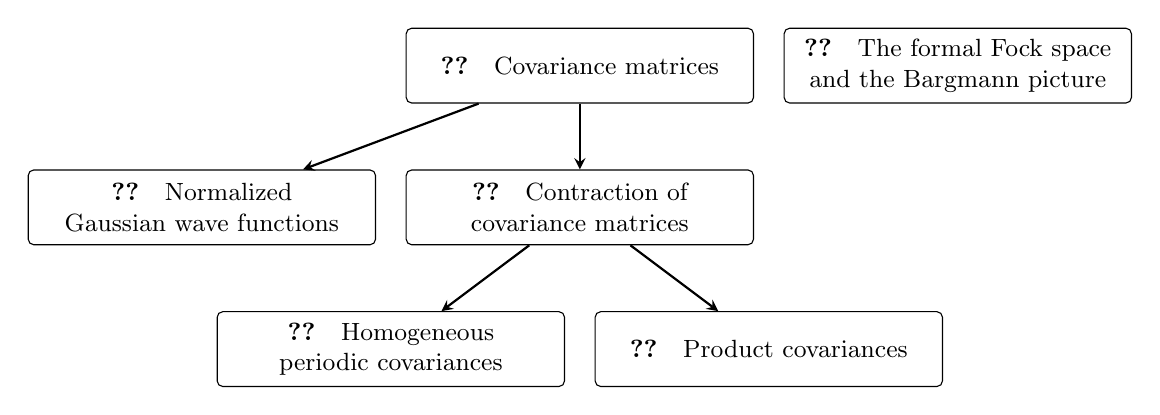
\begin{tikzpicture}[font=\small,
  sec/.style={draw, rounded corners=2pt, text width=4.2cm, align=center, minimum height=0.95cm,
    inner sep=3pt, execute at begin node={\hyphenpenalty=10000}},
  dep/.style={->, >=stealth, thick}]
  \node[sec] (s1) at (0,0) {\ref*{sec:covariance}\quad Covariance matrices};
  \node[sec] (s2) at (-4.8,-1.8) {\ref*{sec:states}\quad Normalized Gaussian wave functions};
  \node[sec] (s3) at (0,-1.8) {\ref*{sec:contraction}\quad Contraction of covariance matrices};
  \node[sec] (s4) at (-2.4,-3.6) {\ref*{sec:fourier}\quad Homogeneous periodic covariances};
  \node[sec] (s5) at (2.4,-3.6) {\ref*{sec:products}\quad Product covariances};
  \node[sec] (s6) at (4.8,0) {\ref*{sec:fock}\quad The formal Fock space and the Bargmann picture};
  \draw[dep] (s1) -- (s2);
  \draw[dep] (s1) -- (s3);
  \draw[dep] (s3) -- (s4);
  \draw[dep] (s3) -- (s5);
\end{tikzpicture}}
\caption{\revs{Dependence of the sections. An arrow means that the later section uses the earlier
one; arrows implied by a chain of arrows are omitted. Section~\ref{sec:states} enters
Sections~\ref{sec:contraction} and~\ref{sec:products} only in remarks, and Section~\ref{sec:fock}
uses no other section.}}
\label{fig:roadmap}
\end{figure}
